\begin{center}
	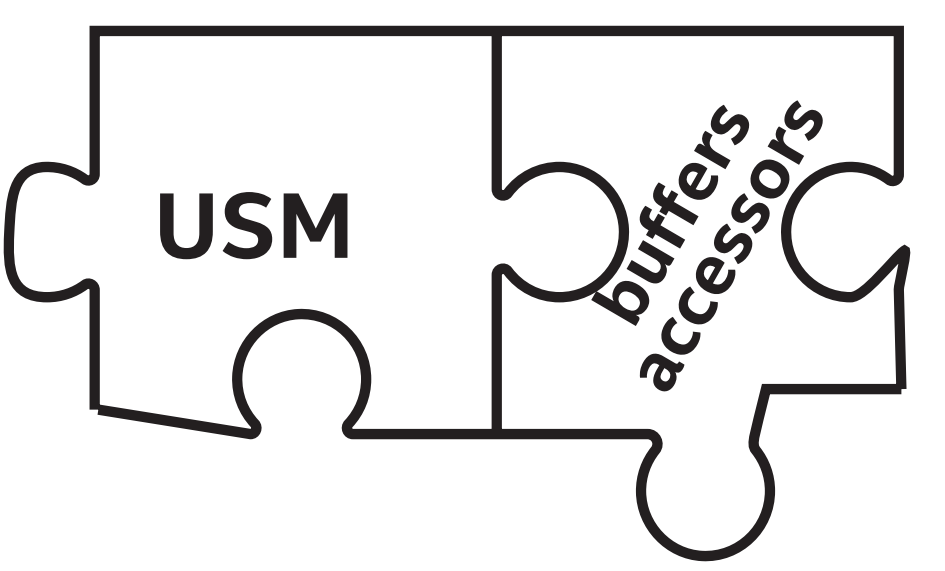
\includegraphics[width=0.5\textwidth]{content/chapter-3/images/1}
\end{center}

超级计算机的架构师们经常哀叹,我们需要“喂养野兽”。“喂野兽”指的是在使用大量并行的计算机的“野兽”,向它喂数据成了需要解决的关键性挑战。\par

在异构机器上提供数据并行C++程序,需要确保数据在需要时在正确的地方。大的程序中,可能会有很多工作。而在一个C++程序中,整理出如何管理所有需要的数据移动就可能是一场噩梦。\par

我们将解释管理数据的两种方法:统一共享内存(Unified Shared Memory, USM)和缓冲区。USM是基于指针的,C++开发者对它很熟悉。缓冲区提供了更高级别的抽象。\par

我们需要控制数据的移动,本章将介绍实现该目标的方式。\par

第2章中,我们研究了如何控制代码的执行位置。代码需要数据作为输入,生成数据作为输出。因为代码可能运行在多个设备上,而这些设备不一定共享内存,所以需要管理数据移动。即使数据是共享的,比如USM,同步和一致性也是需要理解和管理的。\par

一个合乎逻辑的问题是“为什么编译器不自动地做所有的事情?”我们可以自动处理很多事情,但如果不把自己定位为开发者,性能通常是次优的。在实践中,为了获得最佳性能,编写异构程序时,需要关注代码执行(第2章)和数据移动(本章)。\par

本章提供了管理数据的介绍,包括数据使用的顺序。前一章展示了如何控制代码的运行位置,本章将让数据显示在我们要求代码执行的地方,这不仅对正确执行应用程序很重要,而且也可以最小化执行时间和功耗。\par








